%% Submissions for peer-review must enable line-numbering 
%% using the lineno option in the \documentclass command.
%%
%% Preprints and camera-ready submissions do not need 
%% line numbers, and should have this option removed.
%%
%% Please note that the line numbering option requires
%% version 1.1 or newer of the wlpeerj.cls file, and
%% the corresponding author info requires v1.2

\documentclass[fleqn,10pt,lineno]{wlpeerj} % for journal submissions
% \documentclass[fleqn,10pt]{wlpeerj} % for preprint submissions

\usepackage{float}
\floatplacement{figure}{H}
\title{Spatial variation in allometric growth of invasive lionfish has
management implications}

\author[1]{Juan Carlos Villaseñor-Derbez}
\author[1]{Sean Fitzgerald}
\affil[1]{Bren School of Environmental Sciences and Management, University of California
  Santa Barbara, Santa Barbara, California, USA}
\corrauthor[1]{Juan Carlos Villaseñor-Derbez}{juancarlos@ucsb.edu}

\keywords{Lionfish, invasive species, length-weight, allometric, regional variations}

\begin{abstract}
Lionfish (\textit{Pterois volitans / miles}) are an invasive species in
the Western Atlantic and the Caribbean. Improving management of invasive
lionfish populations requires accurate total biomass estimates, which
depend on accurate estimates of allometric growth, but sedentary species
like lionfish often exhibit high levels of spatial variation in life
history characteristics. We reviewed 17 published length-weight
relationships for lionfish taken throughout their invasive range and
found regional differences that led to significant misestimates when
calculating weight from length observations. The spatial pattern we
observed is consistent with findings from other studies focused on
genetics or length-at-age. Here, the use of \textit{ex situ} parameter
values resulted in total biomass estimates between 76.2\% and 140\% of
true observed biomass, and up to a threefold under- or overestimation of
total weight for an individual organism. These findings can have
implications for management in terms of predicting effects on local
ecosystems, evaluating the effectiveness of removal programs, or
estimating biomass available for harvest.
\end{abstract}

\begin{document}

\flushbottom
\maketitle
\thispagestyle{empty}

\section*{Introduction}

Lionfish (\emph{Pterois volitans/miles} complex) are an invasive species
in the Western Atlantic Ocean and Caribbean Sea, likely introduced
through release of aquarium-kept organisms \citep{betancurr_2011}.
Lionfish are the first invasive marine vertebrates established along
these coasts \citep{schofield_2009,schofield_2010,sabidoitza_2016}, and
they have established invasive populations in coral reefs, estuaries,
mangroves, hard-bottomed areas, and mesophotic reefs
\citep{barbour_2010,jud_2011,muoz_2011,claydon_2012,andradibrown_2017,gress_2017}.
Their presence has been labeled as a ``major marine invasion'' because
they threaten local biodiversity, spread rapidly, and are difficult to
manage \citep{hixon_2016}.

A substantial amount of research describes lionfish impacts throughout
their invaded range. A meta-analysis by \citet{peake_2018} showed that
invasive lionfish prey on at least 167 different species across the
tropical and temperate Western Atlantic. Their feeding behavior and high
consumption rates can reduce recruitment and population sizes of native
reef-fish species, and can further endanger reef fish
\citep[][but see \citealt{hackerott_2017} for a counterexample]{green_2012,rocha_2015}.
For example, field experiments showed that lionfish establishment in the
Bahamas led to reduced recruitment of native fishes by nearly 80\% over
a five-week period \citep{albins_2008}, and prey fish biomass declined
by 65\% over two years as lionfish biomass increased along Bahamian
coral reefs \citep{green_2012}. However, trophic impacts of lionfish can
be minimized if their local biomass is controlled by culling
\citep{ariasgonzalez_2011}.

Governments and non-profit organizations have sought to reduce lionfish
densities through removal programs and by incentivizing its consumption
\citep{chin_2016}. In some cases, these have shown to significantly
reduce -- but not quite eliminate -- lionfish abundances at local scales
\citep{deleon_2013,sandel_2015}. Complete eradication of lionfish
through fishing is unlikely because of their rapid recovery rates and
ongoing recruitment to shallow-water areas from persistent populations
in mesophotic ecosystems \citep{barbour_2011,andradibrown_2017}.
However, promoting lionfish consumption might create a level of demand
capable of incentivizing a stable fishery while controlling
shallow-water populations, thus creating alternative livelihoods and
avoiding further negative effects to local biota.

The feasibility of establishing fisheries through lionfish removal
programs has been extensively evaluated through field observations and
empirical modeling
\citep{barbour_2011,morris_2011,deleon_2013,johnston_2015,sandel_2015,usseglio_2017}.
Determining the feasibility of such initiatives requires modeling the
change in biomass in response to changes in fishing mortality
(\emph{i.e.,} culling). A common way to model this is via
length-structured population models, where fish lengths are converted to
weight to calculate total biomass
\citep{barbour_2011,cote_2014,andradibrown_2017}. The allometric
length-weight relationship is thus an essential component of these
models, but this relationship can vary across regions as a response to
biotic and abiotic conditions \citep{johnson_2016}.

Outcomes of previous studies suggest lionfish are likely to exhibit
spatial heterogeneity in the length-weight relationship for both
behavioral and biological reasons. Important life history
characteristics such as growth or natural mortality rates are often
spatially variable for fish that exhibit sedentary behavior
\citep{gunderson_2008,hutchinson_2008,wilson_2012,guan_2013}, and in
fact, high levels of site fidelity and small home ranges are two primary
reasons why culling programs are effective in reducing local adult
lionfish populations
\citep{Fishelson_1997,kochzius_2005,jud_2012,cote_2014}. Genetic
analysis of lionfish also identified two genetically distinct invasive
subpopulations between the Western Atlantic and the Caribbean,
suggesting the existence of spatially explicit biological differences
between populations as well \citep{betancurr_2011}. Site-specific
studies that calculate the length-weight relationship of lionfish report
variable estimates, and these differences may be increasingly important
when estimating the potential effectiveness of lionfish culling programs
\citep{barbour_2011,morris_2011,cote_2014,johnston_2015}. However, the
influence of using \emph{ex situ} parameters when estimating the
length-weight relationship remains unexplored.

Our objective was to quantify the magnitude of error caused by using
\emph{ex situ} parameter values when estimating lionfish weight from
length observations. In this study, we calculated and reported the first
length-weight relationship for lionfish in the central Mexican Caribbean
using previously collected \emph{in situ} observations (n = 109;
\citet{villaseorderbez_2014}). We then estimated lionfish weight in this
area using previously published length-weight relationships for lionfish
populations from ten locations across the Western Atlantic, Gulf of
Mexico, and Caribbean. By comparing these weight estimates to our
\emph{in situ} length-weight observations, we showed that using \emph{ex
situ} parameter values resulted in up to a threefold under- or
overestimation of lionfish weight and estimated of total biomass ranged
between 76\% and 140\% of observed total biomass.

\section*{Methods}

We reviewed 12 published studies and obtained 17 length-weight
relationships for the Western Atlantic (n = 2), Gulf of Mexico (n = 7),
and Caribbean (n = 8, Table \ref{tab:all_params}, Fig \ref{fig:map}).
Study sites included North Carolina, the Northern and Southern Gulf of
Mexico, the Southern Mexican Caribbean, the Bahamas, Little Cayman,
Jamaica, Bonaire, Puerto Rico, and Costa Rica
\citep{barbour_2011,darling_2011,deleon_2013,fogg_2013,dahl_2014,edwards_2014,toledohernndez_2014,sandel_2015,aguilarperera_2016,sabidoitza_2016,sabidoitz_2016,chin_2016}.
We have access only to the summarized information published in these
studies - not the raw data authors used to make length-weight
calculations. We collected information on sex differentiation, location,
length and depth ranges, and sampling methods from each study when
available. Only two studies reported sex-specific length-weight
parameters \citep{aguilarperera_2016,fogg_2013}, so we assumed data were
reported for both sexes combined in all other studies. Reviewed studies
presented information for organisms ranging from 25-475 mm in Total
Length (\(TL\)) and were obtained at depths between 0.5 m and 57 m. Four
studies explicitly stated that their organisms were sampled with pole
spears \citep{dahl_2014,aguilarperera_2016,chin_2016,sabidoitz_2016},
and six studies mentioned that some of their organisms were obtained
with pole spears (or other type of harpoon) but also hand-held nets or
fish traps
\citep{barbour_2011,fogg_2013,edwards_2014,toledohernndez_2014,sandel_2015,sabidoitza_2016}.
Two studies did not specify how organisms were sampled
\citep{darling_2011,deleon_2013}.

We also used data from 109 lionfish sampled by
\citet{villaseorderbez_2014}, who used hand nets and numbered bottles to
collect Total Length (TL; mm) and Total Weight (TW; g) for organisms
from 10 sampling sites along the central Mexican Caribbean coast in the
Summer of 2010 (Supplementary Table 1). Sampling locations included wall
and carpet reefs at depths between 5.7 m and 38.1 m. The use of hand
nets prevented any weight loss due to bleeding and allowed better
representation of small sizes by avoiding gear selectivity. Organisms
were euthanized via pithing.

\begin{figure}
\centering
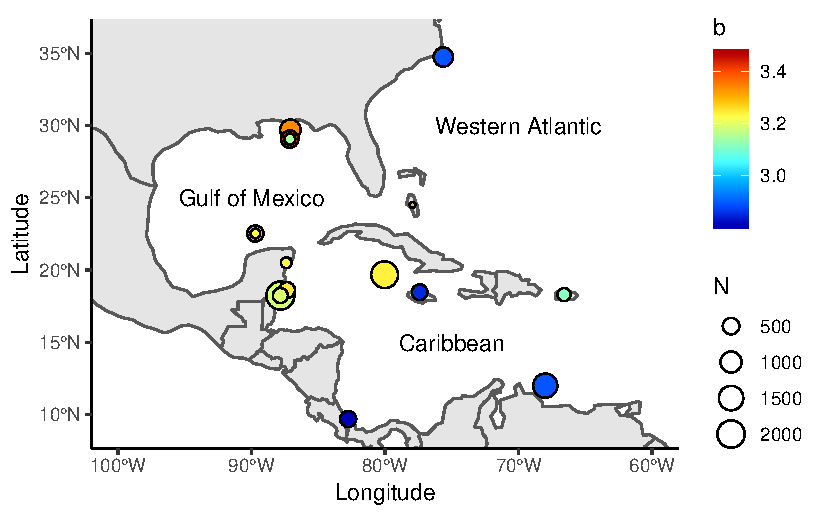
\includegraphics{Manuscript_files/figure-latex/map-1.pdf}
\caption{\label{fig:map}Locations where allometric growth parameters of
lionfish (\emph{Pterois spp}) have been reported. Circle sizes indicate
sample size from each study, colors indicate the \(b\) coefficient from
Eq. \ref{eq:allometric}.}
\end{figure}

The weight-at-length relationship for lionfish in the central Mexican
Caribbean was calculated with the allometric growth function:

\begin{equation}
\label{eq:allometric}
TW = aTL^b
\end{equation}

Where \(a\) is the ponderal index and \(b\) is the scaling exponent or
allometric parameter. We linearized the equation using
\(log_{10}\)-transformation and estimated the coefficients using an
Ordinary Least Squares Regression with a heteroskedastic-robust standard
error correction \citep{zeileis_2004}. Coefficients were tested with a
two-tailed Student's t-test, and the significance of the regression was
corroborated with an F-test. Some of the reviewed studies (Table
\ref{tab:all_params}, Fig \ref{fig:map}) inconsistently defined \(a\) as
either the ponderal index from Eq. \ref{eq:allometric} or the
y-intercept from the linearized log-transformed equation. Other studies
incorrectly reported parameters as mm-to-g conversions when they were in
fact cm-to-g conversions. We standardized each study by converting
coefficients and report all parameters as TL (mm) to TW (g) conversions.

We obtained a total of 18 parameter pairs by combining length-weight
parameters extracted from the literature and the additional pair
calculated here (Fig \ref{fig:all_allo}). Recall that the objective of
this study is not to describe differences in the length-weight
relationship between populations (which would require access to raw
data), but rather to assess how \emph{ex situ} parameter values
influence the accuracy of weight estimates for lionfish, using the
central Mexican Caribbean as a case study. Using each of the 18
parameter pairs, we estimated \(TW\) from the \(TL\) observations
collected in the central Mexican Caribbean (n = 109, with \(TL\) ranging
from 34 mm to 310 mm) and divided predicted weights by known observed
weights to obtain a simple measure of over- or underestimation.
Difference in mean weight ratios were tested with an analysis of
covariance (ANCOVA):

\begin{equation}
R_{i,j} = \tilde{\mu} + \alpha_j + \beta TL_{ij} + e_{ij}
\end{equation}

\clearpage

Where \(R_{ij}\) is the weight ratio for the \(i\)-th organism obtained
with parameters from the \(j\)-th study, \(\tilde{\mu}\) is a constant
for all individuals, \(a_j\) is the treatment effect (\emph{i.e.,} the
difference induced by each study), \(TL_{ij}\) is the covariate
(\emph{i.e.,} Total Length) for the \(i\)-th subject in the \(j\)-th
group with slope \(\beta\), and \(e_{ij}\) is the error term of the
regression. Ratios were logit-transformed prior to analysis, and a
\emph{post-hoc} Tukey's test was used to identify groups where mean
ratios did not differ. All analyses were performed in R version 3.5.2
\citep{rcore_2018}. Raw data and code used in this work are available on
github at github.com/jcvdav/lionfish\_biometry.

\begin{table}[!h]

\caption{\label{tab:unnamed-chunk-2}\label{tab:all_params}Summary of 18 allometric growth parameters available for lionfish in the invaded range from peer-reviewed literature and this study. All parameters have been adjusted to convert from millimeters to grams. n = Sample size, Sex specifies whether data was presented for Females (F), Males (M), or both sexes combined (B), a = scaling parameter (presented in $\times 10^{-5}$), b = exponent.}
\centering
\begin{tabular}{llllrll}
\toprule
Region & Sex & n & a & b & $R^2$ & Reference\\
\midrule
Western Atlantic & B & 774 & 2.90 & 2.89 & - & Barbour et al., 2011\\
Western Atlantic & B & - & 0.25 & 3.29 & - & Darling et al., 2011\\
GoM & B & 934 & 0.21 & 3.34 & 0.98 & Dahl \& Patterson, 2014\\
GoM & B & 472 & 0.29 & 3.30 & 0.95 & Aguilar-Perera \& Quijano-Puerto, 2016\\
GoM & F & 67 & 0.12 & 3.47 & 0.95 & Aguilar-Perera \& Quijano-Puerto, 2016\\
GoM & M & 59 & 0.42 & 3.23 & 0.95 & Aguilar-Perera \& Quijano-Puerto, 2016\\
GoM & B & 582 & 0.14 & 3.43 & 0.99 & Fogg et al., 2013\\
GoM & M & 119 & 0.27 & 3.31 & 0.97 & Fogg et al., 2013\\
GoM & F & 115 & 0.68 & 3.14 & 0.94 & Fogg et al., 2013\\
Caribbean & B & 458 & 3.60 & 2.81 & - & Sandel et al., 2015\\
Caribbean & B & 419 & 2.80 & 2.85 & 0.87 & Chin et al., 2016\\
Caribbean & B & 1450 & 2.30 & 2.89 & 0.92 & de Leon et al., 2013\\
Caribbean & B & 1887 & 0.30 & 3.24 & 0.97 & Edwards et al., 2014\\
Caribbean & B & 2143 & 0.52 & 3.18 & 0.99 & Sabido-Itza et al., 2016\\
Caribbean & B & 227 & 0.80 & 3.11 & 0.96 & Toledo-Hernández et al., 2014\\
Caribbean & B & 449 & 0.23 & 3.25 & 0.97 & Sabido-Itza et al., 2016b\\
Caribbean & B & 368 & 0.32 & 3.19 & 0.98 & Sabido-Itza et al., 2016b\\
Caribbean & B & 109 & 0.32 & 3.23 & 0.98 & This study\\
\bottomrule
\end{tabular}
\end{table}

\clearpage

\section*{Results}

The length-weight relationship for organisms from the central Mexican
Caribbean (Fig \ref{fig:l-w-carib}) resulted in coefficient values of
\(a = 3.205 \times 10^{-6}\) and \(b = 3.235\) (\(R^2 = 0.977\),
\(F_{1, 107} = 6928.67; p < 0.001\)). The allometric factor (\(b\)) was
significantly different from \(b = 3\) (\(t_{107} = 6.04; p<0.001\)),
corroborating that lionfish present allometric growth. The length-weight
coefficients estimated here were within the range identified by studies
from other regions (Table \ref{tab:all_params}).

\begin{figure}
\centering
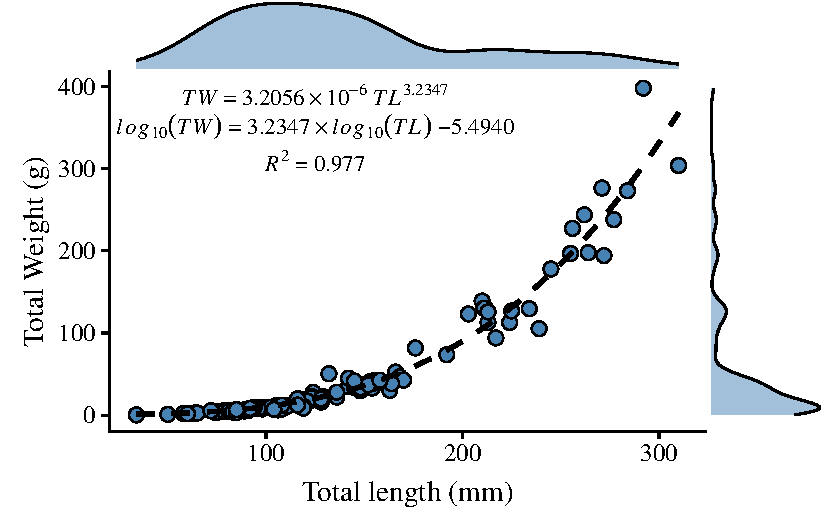
\includegraphics{Manuscript_files/figure-latex/fit1-1.pdf}
\caption{\label{fig:l-w-carib}Length-weight relationship for 109
lionfish sampled in the central Mexican Caribbean. Points indicate
samples, dashed black line indicates curve of best fit, marginal plots
represent the density distribution of each variable.}
\end{figure}

ANCOVA results revealed significant differences in our predicted weight
ratios for the central Mexican Caribbean when using each of the
different pairs of parameters (\(F_{17, 1943} = 24.96; p < 0.001\); Fig
\ref{fig:bio_ratio}). For example, the actual observed weights of the
109 lionfish from the Central Mexican Caribbean had a mean \(\pm\) SD of
52.56 \(\pm\) 76.58 g. However, if we used allometric parameter values
from Banco Chinchorro in the Caribbean to predict weights from our
observed length observations, we estimated a mean \(\pm\) SD of 40.37
\(\pm\) 58.74 g \citep{sabidoitz_2016}. If we similarly used parameter
values from North Carolina in the Western Atlantic to estimate lionfish
weights in the Central Mexican Caribbean, we found a mean \(\pm\) SD of
73.76 \(\pm\) 96.11 g \citep{barbour_2011}. Weights predicted from these
extreme parameters correspond to mean predicted-to-observed weight
ratios of 0.80 \(\pm\) 0.19 and 1.76 \(\pm\) 0.50 (mean \(\pm\) SD),
respectively. Furthermore, largest errors for individual organisms
collected in the central Mexican Caribbean resulted in ratios of 0.36
and 3.51 (\emph{i.e.,} the tails of each violin in Fig
\ref{fig:bio_ratio}). If we examined biomass (\emph{i.e.,} summing
across all 109 organisms) instead of mean ratios, total biomass
estimates were 76.2\% (4,363.53 g) and 140\% (8,039.96 g) of true
observed biomass (5,729.34 g). Parameters for this study estimate total
biomass at 98\% of observed biomass. These misestimates come from the
two most extreme sets of parameters, but results varied consistently
across locations (Figs \ref{fig:bio_ratio} and \ref{fig:errors}).
Overall, the use of \emph{ex situ} parameters led to significantly
erroneous estimates of individual weight and total biomass for lionfish.

Tukey's \emph{post-hoc} test showed that weight ratios for the central
Mexican Caribbean differeed from those obtained with parameters from the
Western Atlantic, and most sites in the Caribbean and the Gulf of Mexico
(Tukey's HSD \(p > 0.05\)). The only sites where weight ratios did not
differ from the central Mexican Caribbean were Little Cayman
\citep{edwards_2014}, Bahamas \citep{darling_2011},
and the Northern Gulf of Mexico (\citet{dahl_2014}; Tukey's HSD
\(p > 0.05\)). All weight estimates using parameters from the Gulf of
Mexico and Western Atlantic were higher than observed values, and only
parameters from the Caribbean produced weights smaller than observed
(Fig \ref{fig:bio_ratio}). The regional average (\(\pm\) SD) of
predicted-to-observed weight ratios from these three regions were 1.24
\(\pm\) 0.309, 1.41 \(\pm\) 0.523, and 1.20 \(\pm\) 0.423 for the Gulf
of Mexico, Western Atlantic, and Caribbean, respectively. This suggests
that the smallest errors are observed when using parameters from other
locations in the Caribbean.

\begin{figure}
\centering
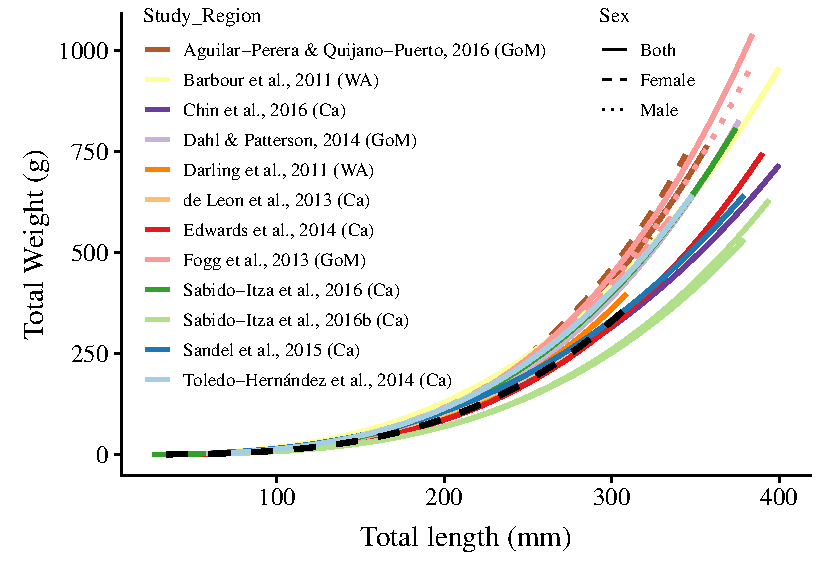
\includegraphics{Manuscript_files/figure-latex/fit2-1.pdf}
\caption{\label{fig:all_allo}Length-weight relationships (n = 18) for 12
studies and this study. The curves are shown for the range of lengths
reported in each study (See Supplementary Table 2); when ranges were not
present, we use the ones found in this study (34 mm - 310 mm). Colors
indicate studies from which the parameters were extracted. Dotted,
dashed, and solid lines show models for males, females, and combined
sexes, respectively. Letters in parentheses indicate if the study comes
from the Gulf of Mexico (GoM), Western Atlantic (WA), or Caribbean (Ca).
The dashed black line represents the relationship estimated in this
study. There are two solid green lines for Sabido-Itza et al, 2016b, one
for each of the two sites for which they report parameters. A log-log
version of this figure is presented in Figure S4.}
\end{figure}

\begin{figure}
\centering
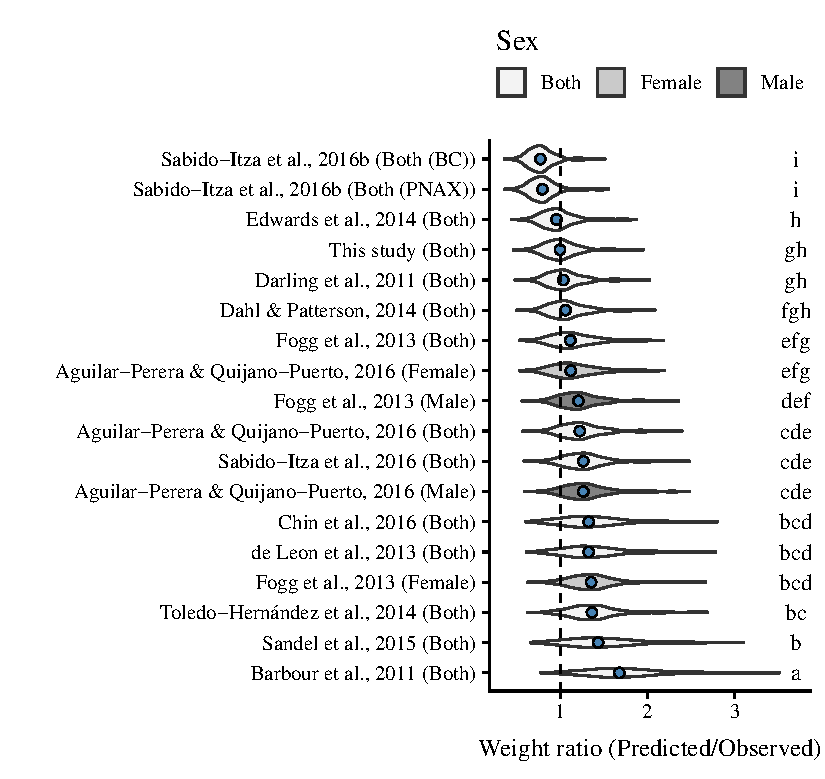
\includegraphics{Manuscript_files/figure-latex/pred_obs-1.pdf}
\caption{\label{fig:bio_ratio}Violin plot of predicted-to-observed
weight ratios when applying each of 18 different pairs of allometric
parameters to the 109 lionfish collected in the central Mexican
Caribbean. Sex is indicated in parentheses. Blue circles indicate median
values and like letters indicate values that do not differ
significantly. For Sabido-Itza et al, 2016b, BC and PNAX make reference
to Banco Chinchorro and Parque Nacional Arrecifes de Xcalak, two sites
for which they report parameters.}
\end{figure}

\begin{figure}
\centering
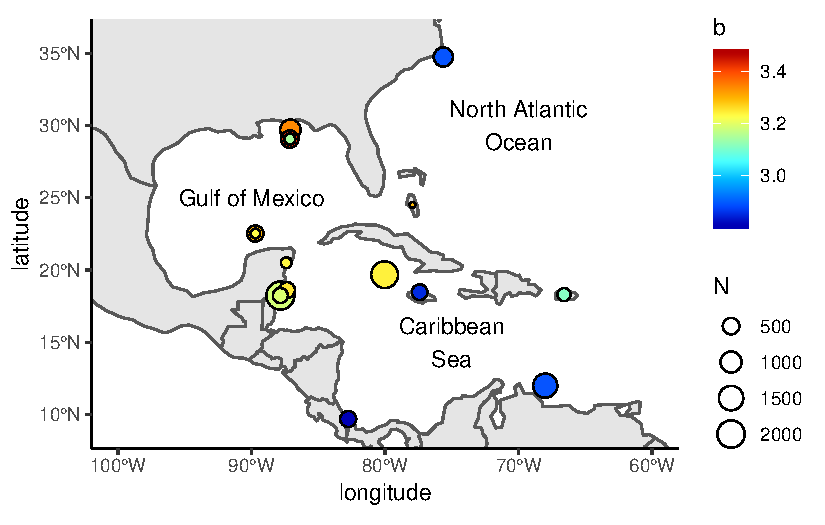
\includegraphics{Manuscript_files/figure-latex/unnamed-chunk-9-1.pdf}
\caption{\label{fig:errors}Estimated total biomas relative to observed
biomass (5,729.34 g) for 18 pairs of allometric parameters. Sex is
indicated in parentheses. For Sabido-Itza et al, 2016b, BC and PNAX make
reference to Banco Chinchorro and Parque Nacional Arrecifes de Xcalak,
two sites for which they report parameters.}
\end{figure}

\clearpage

\section*{Discussion}

Our results suggest that lionfish exhibit highly variable, spatially
heterogeneous allometric relationships across their invaded range, and
that this variation is relevant for managing invasions. Moreover, we
show that the use of \emph{ex situ} parameter values may lead to highly
biased weight and total biomass estimates. Our comparison of observed
weights to those predicted with locally-informed parameters and \emph{ex
situ} parameters showed that weight of an individual lionfish can be
overestimated by more than threefold, highlighting the need to use local
information. Here we discuss the implications of our findings, possible
shortcommings in our analyses, and highlight potential future research
directions.

Differences in length-weight relationships have traditionally been
highlighted as potential pitfalls to fishery management. For example,
\citet{wilson_2012} showed that small-scale variations in length-at-age
and fishing mortality in other Scorpaeniformes translate to differential
landings, effort, and catch per unit effort in the live fish fishery of
California, and that these differences must be taken into account in
management plans. The lionfish case poses the opposite scenario, where
the manager desires to eradicate the species. To accurately gauge both
the effectiveness of lionfish removal efforts and the resources needed
to successfully manage an invasion, we must acknowledge and understand
regional biological differences in important variables such as
allometric growth parameters.

We detected substantial differences in weight-at-length between
organisms from the Caribbean, Gulf of Mexico, and Western Atlantic.
Groupings of predicted-to-observed weight ratios identified in our
\emph{post hoc} testing aligned with the spatial distribution of the
examined studies, suggesting that these differences may be mediated by
space. These regional allometric differences mirror similar patterns in
length-at-age of lionfish across both their invaded and native regions
\citep{pusack_2016}. Variation may be driven by genetics or by
organisms' exposure to distinct environmental conditions. For example,
\citet{betancurr_2011} used mitochondrial DNA to demonstrate the
existence of two distinct population groups, identified as the
``Caribbean group'' and ``Northern Group'', and \citet{fogg_2015}
alternatively suggested that length-at-age differences may be driven by
the environment.

One might be inclined to attribute all variation in the lionfish
length-weight relationship to the spatial origin of these parameters.
However, samples from the 12 studies included here were not only
collected in different locations, but also at different points in time
and across different depth and size ranges (See Supplementary Table 2
for an extended version of Table 1). The magnitude of the bias
discovered in this study and our lack of understanding the sources
driving spatial variation for lionfish highlights the need to
simultaneously collect length-weight information across the invaded
range to test for spatially-induced patterns and to link these findings
to previously suggested environmental and genetic structures. Such an
endeavor would provide insight into lionfish biology and better inform
management. However, while we could not evaluate how these factors
influenced length-weight estimates from previous studies without raw
data, we still show that a lack of locally-calculated parameters can
induce significant bias when calculating weight from length
observations. We demonstrate the importance of using \emph{in situ}
parameters to obtain accurate weight estimates regardless of the
underlying mechanisms driving variation between populations.

Applying parameter estimates to lengths outside the range of lengths
originally used to estimate the parameters may also induce error. Our
smallest observed organism was 34 mm in \(TL\), and only two studies
estimated parametrs with smaller organisms
\citep{edwards_2014,sabidoitza_2016}. By contrast, our largest organism
had a \(TL\) of 310 mm, which is well within the range of all other
studies (the next smallest maximum length was 325 mm; See Supplementary
Table 2). Due to the power function describing the allometric
relationship (\emph{i.e.,} Eq. 1), the error in weight estimates is
larger when extrapolation is done for lengths that are larger than the
maximum length used to estimate the parameters. Our estimates are
therefore conservative because we only used parameter pairs from other
studies to estimate weights for lionfish up to 310 mm in the Central
Mexican Caribbean, well within the range of lengths for which other
parameters were estimated.

The results presented here have key implications for management. For
example, \citet{edwards_2014} simulated a lionfish culling program under
two scenarios, one using length-at-age and length-to-weight parameters
from North Carolina and one using parameters from Little Cayman. Their
results show that using different parameters caused up to a four-year
difference in the time required for the simulated lionfish population to
recover to 90\% of its initial biomass after removals ceased. Here, we
show that using one set of length-weight parameters versus another for a
given length can result in more than a threefold under- or
overestimation of total weight for individual fish, and that total
biomass estimates may range between 76\% and 140\% of true observed
biomass. These differences become especially important when allocating
resources for lionfish removal programs, incentivizing lionfish
fisheries as a source of alternative livelihoods, or estimating
ecosystem impacts. Research efforts focused on invasive lionfish
populations need to use parameters calculated for their region to the
extent possible, or use different sets of parameters that provide
appropriate upper and lower bounds in their results.

\section*{Acknowledgements}

We thank Nils Van Der Haar and Michael Doodey from Dive Aventuras as
well as Guillermo Lotz-Cador who provided help to collect samples. We
are grateful for comments raised by the editor and two anonymous
reviewers, which significantly increased the quality of this work.

Conflict of Interest: The authors declare that they have no conflict of
interest.

\bibliography{references}

\end{document}